\documentclass[10pt,twocolumn,letterpaper]{article}

\usepackage{iccv}
\usepackage{times}
\usepackage{epsfig}
\usepackage{graphicx}
\usepackage{amsmath}
\usepackage{amssymb}
\usepackage{subcaption}

% Include other packages here, before hyperref.

% If you comment hyperref and then uncomment it, you should delete
% egpaper.aux before re-running latex.  (Or just hit 'q' on the first latex
% run, let it finish, and you should be clear).
\usepackage[breaklinks=true,bookmarks=false]{hyperref}

\iccvfinalcopy % *** Uncomment this line for the final submission

\def\iccvPaperID{****} % *** Enter the ICCV Paper ID here
\def\httilde{\mbox{\tt\raisebox{-.5ex}{\symbol{126}}}}

% Pages are numbered in submission mode, and unnumbered in camera-ready
%\ificcvfinal\pagestyle{empty}\fi
\setcounter{page}{4321}
\begin{document}

%%%%%%%%% TITLE
\title{Multispectral Texture characterization: Application to Mitotic Count in Breast Cancer Histopathology}

\author{Humayun Irshad, Ludovic Roux\\
University Joseph Fourier Grenoble, France\\
{\tt\small {humayun.irshad, ludvoic.roux}@ipal.cnrs.fr} \\
\and 
Alexandre Gouallard\\
Institution2\\
First line of institution2 address\\
{\tt\small secondauthor@i2.org} \\
\and
Daniel Racoceanu\\
University Pierre and Marie Curie\\
France\\
{\tt\small daniel.racoceanu@upmc.fr}
}

\maketitle
%\thispagestyle{empty}

%%%%%%%%% ABSTRACT
\begin{abstract}
Multispectral Imaging (MSI) ...
\end{abstract}

%%%%%%%%% BODY TEXT
\section{Introduction}
%Medical (Scanner, big objects, not to many) vs Biology/biomedical (microscopic, small objects, large in quantity)

In medical imaging, computer aided detection (CADe), also called computer aided diagnosis (CADx) systems have played a significant part in medicine that assist doctors in interpretation of medical images. CAD systems are extensively used in the detection and differential diagnosis of many different types of abnormalities in medical images obtained using different imaging modalities. Medical imaging can be divided into radiology and pathology. Both the imaging modalities look for anatomical or physiological reasons for injury or disease. A radiologist is trained to review x-ray, and other non-invasive images and scans of the anatomical object like brain, lung, heart (e.g., ultrasound or MRI) for diagnosis. A large amount of research are available on CAD in radiology including different image modalities like x-rays, ultrasound, MRI, CT and mammogram ~\cite{sonka2000,bankman2000,erickson2002,summers2003,giger2004}. The pathologist is also trained to perform such evaluation on biological objects, but with actual tissue samples. The standard computer vision methodology are employed in mostly CAD systems involved object detection, segmentation and classification. However, in the recent years, CAD systems in pathology is an active area of research and posing more challenging problem as compared to radiology where pathologists traditionally make a diagnostic decision by viewing a specimen under microscope and measuring various diagnostically important attributes of an isolated object such as size, shape, darkness, color and texture.

Image processing and computer vision techniques are of special interest for pathologists because they can be more reliable than classical assessment by eye screening using poorly defined criteria. Being important in diagnostic pathology, this qualitative assessment is also used to understand the ground realities for specific diagnostic being rendered like specific chromatin texture in cancerous nuclei, which may indicate certain genetic abnormalities. In addition, quantitative characterization of pathology imagery is important not only for clinical applications (e.g., to reduce/eliminate inter- and intra-observer variation in diagnosis) but also for research applications (e.g., to understand the biological mechanisms of the disease process~\cite{gurcan2009}. 

Histopathological study has been conducted for numerous cancer detection and grading applications including brain~\cite{ alkadi2010, sertel2009}, breast~\cite{ petushi2006,dundar2011,basavanhally2012},cervix~\cite{ Keenan2000} etc. One of the most difficult fields in histopathology imagery is spatial analysis, more specifically automated nuclei detection and classification. The objective of nuclei classification is assign label to different type of nuclei as normal, cancer, mitotic, apoptosis, lymphocytes etc that in particular, a challenging problem to address in histopathology. H\&E is a well established staining technique in histopathology that exploits intensity of stains in the tissue images to quantify the nuclei and other structures related to cancer developments. Image processing techniques in this context are devoted to the accurate and objective quantification and localization of such activity in specific regions of the tissue such as cytoplasm, membranes and nuclei. During the last decade, a large amount of research has focused on histology imagery, which raised much challenging imaging problems than with cytology imagery. There are several strategies for nuclei classification in color (RGB) histological images that lack in accuracy due to the process of acquisition (slicing, staining, teering, etc) creates poor 3D correlation in image color, gradient and structures.

Pathology provides the critical link between the biological basis of an image or spectral signature and clinical outcomes obtained through optical imaging. The validation of optical images and spectra requires both morphologic diagnosis from histopathology and parametric analysis of tissue features above and beyond the declared pathologic diagnosis ~\cite{wells2007}. From the chromatic viewpoint, nuclear regions are characterized by non-uniform stain intensity and color, thus preventing a trivial classification based on color separation. In fact, the superposition of tissue layers as well as the diffusion of the dyes on the tissue surface may bring the stains to contaminate the background or other cellular regions which are different from their specific target. Moreover, different portions of the same tissue are may be not equally enlightened and stained. Indeed, multispectral images will allow biologists and pathologists to see beyond the RGB image planes that they are accustomed to. 

Multispectral imaging (MSI) is currently in a period of transition from its role as an exotic technique to its being offered in one form or another by all the major microscopy manufacturers. MSI captures images with accurate spectral content correlated with spatial information and reveals the chemical and anatomic features of histopathology. This is because it provides solutions to some of the major challenges in fluorescence-based imaging, namely ameliorating the consequences of the presence of autofluorescence and the need to easily accommodate relatively high levels of signal multiplexing. MSI, which spectrally characterizes and computationally eliminates autofluorescence, enhances the signal-to-background dramatically, revealing otherwise obscured targets. While this article concentrates on detection of mitotic figures in multispectral images, the intent is to showcase the advantages of multispectral imaging in general. 

The reminder of the paper is organized as follows. Section~\ref{sec:previous} reviews the state-of-the-art multispecttral methods, particularly in object or region detection in histopathology, related to this research work. Section~\ref{sec:framework} describes the proposed framework for mitotic figure detection. Experiment and results are presented in section~\ref{sec:results}. Finally, the concluding remarks with future work are given in section~\ref{sec:conclusion}.

%Softwares (MicroMSI, Multispec, Gerbil)
%-------------------------------------------------------------------------
\section{Literature Review}
\label{sec:previous}
The main idea of extracting texture from multispectral images is the use of combined spectral and spatial information for discrimination of region or objects. We found few methods in the MSI literature for texture characterization of histopathological images. Some of them employed single band of MSI and other used multiple selected bands of MSI. Fernandez et al. \cite{fernandez2005} coupled high-throughput Fourier transform infra-red (FTIR) spectroscopic imaging of tissue microarrays with statistical pattern recognition of spectra indicative of endogenous molecular composition and demonstrate histopathologic characterization of prostatic tissue. They explicitly defined metrics to consist of spectral features that have a physical significance related to tissue biochemistry and facilitated the measurement of cell types. The approach in \cite{woolfe2006} used hyperspectral images of colon biopsy slides whereby the classification algorithm was based on spectral analysis to discriminate between normal and cancerous biopsies of the colon tissue. In this study of hyper-spectral cancer analysis, they used Laplacian eigenmaps to take into account the non-linear geometry in the design of learning algorithms and evaluated two approaches for spectral feature selection: Haar wavelet packet best bases (active sensing) and random projections.

Masood et al. \cite{masood2009} proposed a colon biopsy classification method based on spatial analysis of hyperspectral image data from colon biopsy samples. Initially, using circular local binary pattern algorithm, spatial analysis of patterns are represented by a feature vector in selected spectral band. Later, classification is achieved using subspace projection methods like principal component analysis, linear component analysis and support vector machine. Boucheron et al. \cite{boucheron2007} presented an analysis of the utility of multispectral versus standard RGB imagery for pixel level classification of nuclei in H\&E stained histopathological images and found that performance differences between single multispectral image bands and single RGB image bands are not statistically significant. 

Khelifi et al. \cite{khelifi2012} proposed a spatial and spectral gray level dependence method in order to extend the concept of gray level co-occurrence matrix by assuming the presence of texture joint information between spectral bands. Malon et al. \cite{malon2013} demonstrated a segmentation based features with convolutional neural networks using additional focal planes and spectral bands for identification of mitotic nuclei in breast cancer histopathology and achieved best classification accuracy (F-measure = 59\%) on multispectral dataset during ICPR context 2013 \cite{roux2013}.

Recently, Wu et al. \cite{wu2012} proposed a multilayer conditional random field model using a combination of low-level cues and high-level contextual information for nuclei separation in high dimensional data set obtained through spectral microscopy. In this approach, the multilayer contextual information was extracted by an unsupervised topic discovery process from spectral images of microscopic specimen, which efficiently helps to suppress segmentation errors caused by intensity inhomogeneity and variable chromatin texture.

In the proposed methodology, we address limitation of the shortcomings in previous works, including (1) comprehensive analysis of multispectral spatial feature vector in all bands rather than single band \cite{masood2009,wu2009,wu2012} and (2) combining spatial feature with multispectral spatial feature vector in order to discriminate mitotic figures from other nuclei and microscopic objects. The main novel contributions of proposed work are: (1) a multispectral spatial and morphology feature vector computation which inherit discriminant information from other nuclei and (2) an projection features from multispectral features vector for classification of mitotic figures in breast cancer histopathological images.

%------------------------------------------------------------------------
\section{Proposed Method}
\label{sec:framework}
\subsection{Dataset}
We evaluated the proposed methodology on multispectral MITOS dataset \cite{mITOS2012}, a freely available mitosis dataset. The data set is made up of 50 high power fields (HPF) coming from five different slides scanned at 40X magnification using a 10 bands multispectral microscope. There are 10 HPFs per slide and each HPF has a size of $512\times512\mu\text{m}^2$ (that is an area of $0.262mm^2$). The spectral bands are all in the visible spectrum. In addition, for each spectral band, the digitization has been performed at 17 different focus planes (17 layers Z-stack), each plane being separated from the other by 500 nm. For one HPF, there are 170 gray scale images (10 spectral bands and 17 layers Z-stack for each spectral band). These 50 HPFs contain a total 322 mitotic cells. The training data set consists of 35 HPFs containing 226 mitotic cells and evaluation data set consists of 15 HPFs containing 98 mitotic cells \cite{roux2013}. Figure \ref{fig:spectral_bands} shows the spectral coverage of each of the 10~spectral bands of the multispectral microscope.

\begin{figure}[t]
	\centering
	\begin{subfigure}[b]{0.5\textwidth}
		\centering
		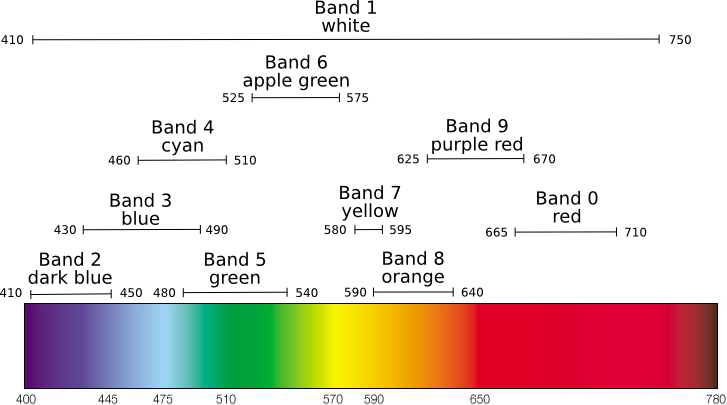
\includegraphics[width=\textwidth]{img/spectral_bands.png}
	\end{subfigure}
	\begin{subfigure}[b]{0.11\textwidth}
		\centering
		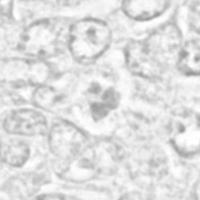
\includegraphics[width=\textwidth]{img/M03_00a_0010_m1.png}
		\caption*{Band 0}
	\end{subfigure}
	\begin{subfigure}[b]{0.11\textwidth}
		\centering
		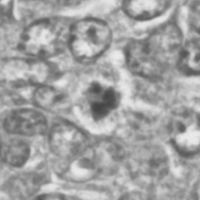
\includegraphics[width=\textwidth]{img/M03_00a_0107_m1.png}
		\caption*{Band 1}
	\end{subfigure}
	\begin{subfigure}[b]{0.11\textwidth}
		\centering
		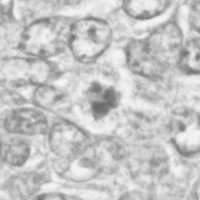
\includegraphics[width=\textwidth]{img/M03_00a_0209_m1.png}
		\caption*{Band 2}
	\end{subfigure}
	\begin{subfigure}[b]{0.11\textwidth}
		\centering
		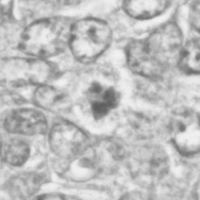
\includegraphics[width=\textwidth]{img/M03_00a_0308_m1.png}
		\caption*{Band 3}
	\end{subfigure}
	\begin{subfigure}[b]{0.11\textwidth}
		\centering
		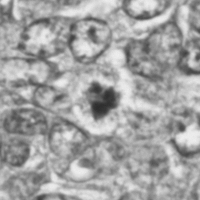
\includegraphics[width=\textwidth]{img/M03_00a_0406_m1.png}
		\caption*{Band 4}
	\end{subfigure}
	\begin{subfigure}[b]{0.11\textwidth}
		\centering
		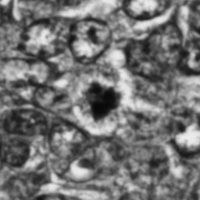
\includegraphics[width=\textwidth]{img/M03_00a_0506_m1.png}
		\caption*{Band 5}
	\end{subfigure}
	\begin{subfigure}[b]{0.11\textwidth}
		\centering
		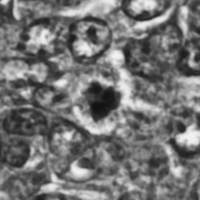
\includegraphics[width=\textwidth]{img/M03_00a_0606_m1.png}
		\caption*{Band 6}
	\end{subfigure}
	\begin{subfigure}[b]{0.11\textwidth}
		\centering
		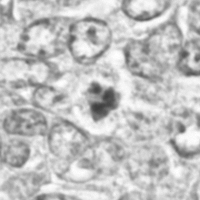
\includegraphics[width=\textwidth]{img/M03_00a_0706_m1.png}
		\caption*{Band 7}
	\end{subfigure}
	\begin{subfigure}[b]{0.11\textwidth}
		\centering
		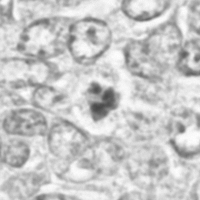
\includegraphics[width=\textwidth]{img/M03_00a_0807_m1.png}
		\caption*{Band 8}
	\end{subfigure}
	\begin{subfigure}[b]{0.11\textwidth}
		\centering
		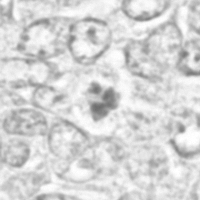
\includegraphics[width=\textwidth]{img/M03_00a_0908_m1.png}
		\caption*{Band 9}
	\end{subfigure}
	\caption{Spectral bands of the multispectral microscope and examples for each band.}
	\label{fig:spectral_bands}
\end{figure}
\subsection{Proposed Method}
In this paper, we propose a mitotic figures detection algorithm based on spatial analysis of multispectral images in breast cancer histopathology. Initially, a z-stack plane is selected based on gradient and band is selected based on histogram analysis. Then, candidates for mitotic figures  are computed on selected band and z-stack plane. A multispectral feature vector is computed for all detected candidates including intensity and texture features in all bands of multispectral images. In addition, using segmented regions of detected candidates, morphological features are also computed. A feature selection algorithm is employed on this multispectral features vector to save the computation cost and to discard any redundancy in the data in order to improve classification accuracy. Classification is achieved using support vector machine (SVM), Bayesian network (BN) as well as decision tree (DT). A side advantage of performing the spatial analysis on a multiple band is to investigate whether improvement in accuracy can be achieved with carefully selected multispectral features to those methods \cite{masood2009,wu2009,wu2012} which use single band data.

%------------------------------------------------------------------------
\section{Experiments and Results}
\label{sec:results}
\subsection{Experiments}

\subsection{Results}

%------------------------------------------------------------------------
\section{Discussion and Conclusion}
\label{sec:conclusion}
%------------------------------------------------------------------------
{\small
\bibliographystyle{ieee}
\bibliography{egbib}
}
\end{document}
